% !TeX root = ../main.tex
\section{Computational cost}
\label{sec:scalability}

% ===========================================================================
% Evidence: Simulations/Scalability/ (rewritten 2026-10-01 for the exact augmented sampler).
%   run_config.R        one (method, n, replicate) per R process, both samplers' own source files with clock reads only
%   run_timing*.sh      sequential drivers;  results/raw/*.rds, results/timing_log.txt
%   profile_mvrnorm.R   dense operations of the Onizuka theta draw in isolation -> results/mvrnorm_profile.csv
%   collect.R, analyze.py -> results/numbers.json, results/table_time_body.tex, figures/scal_*.pdf (copied to figures/)
% Every number below is taken from results/numbers.json, table_time_body.tex or mvrnorm_profile.csv.
% 2026-10-02: wall-time-per-run material removed; the section reports time per sweep and its breakdown only.
% Previous versions of this section: notes/scalability_rewrite_20261001/before/scalability.tex.
% ===========================================================================

This section measures how the time per sweep of Bayesian-PMALA grows with the sample size, where that time is spent, and how it compares with the Laplace and horseshoe Gibbs samplers of \citet{onizuka2024fast}. Both methods use the same normal--exponential augmentation of the asymmetric Laplace likelihood and differ in the trend update: Bayesian-PMALA uses a P-MALA move built from banded linear algebra (Section~\ref{subsec:pmala}), the Onizuka samplers an exact draw from a Gaussian full conditional. The comparison is of running time per Gibbs sweep for the two samplers as implemented.

\paragraph{What a sweep does.} The trend update of Bayesian-PMALA computes the forward and reverse proximal maps by ADMM with a fixed budget of $150$ iterations each and a cold start, using one banded Cholesky factor of the ADMM system shared by both maps and one banded Cholesky factor of the metric $M$ for the proposal noise (Appendix~\ref{app:pmala:admm}); the latent-variable, penalty, interweaving and scale updates act elementwise. Because the iteration budget is fixed, the work of a sweep does not depend on the state of the chain. A sweep of the supplied Onizuka code draws $\theta \sim \mathcal N(A b, \sigma^2 A)$ with $A = (D^\top \Lambda^{-1} D + C)^{-1}$, where $\Lambda$ holds the local scales and $C$ the latent-variable weights, and then updates $\sigma^2$, the $n$ latent variables and the shrinkage parameters. With its \texttt{sparse = TRUE} option, used throughout this section, the precision is assembled by sparse products; R's \texttt{solve} then forms the full dense inverse $A$, and \texttt{MASS::mvrnorm} computes a complete eigendecomposition of $\sigma^2 A$ to form the draw. The default \texttt{sparse = FALSE}, used in Section~\ref{sec:simulations}, performs the same steps and assembles the precision by dense products in addition.

\paragraph{Protocol.} We use the varying-smoothness signal \eqref{eq:sim_vs} with heteroscedastic Gaussian noise, $\tau = 0.5$, $k = 2$, and $n \in \{250, 500, 1000, 2000, 4000\}$; at each $(n, \text{replicate})$ all three samplers receive the same data set. Bayesian-PMALA runs with the default configuration of Section~\ref{subsec:individual}. The Onizuka samplers are the code supplied with that paper, unmodified, with \texttt{sparse = TRUE} and the $\mathrm{IG}(1,1)$ prior on $\sigma^2$ of Section~\ref{sec:simulations}. Both samplers are timed with clock reads inserted at the boundaries of their updates and no other change. All runs were made on one laptop (Intel Core Ultra 7 155U, 32\,GB memory, Windows 11) in R~4.4.1 with its single-threaded reference BLAS, each configuration in a fresh R process pinned to one performance core. For Bayesian-PMALA the time per sweep is the mean over $300$ sweeps that follow the $200$ warm-up sweeps of Appendix~\ref{app:pmala:init} and $100$ sweeps of step-size adaptation, with acceptance rates of $0.40$--$0.49$ in that window. An Onizuka sweep costs too much for windows of that length: we time $30$ sweeps after $5$ at $n = 250$, $20$ after $3$ at $n = 500$, $8$ after $2$ at $n = 1000$, $3$ after $1$ at $n = 2000$, and $2$ after $1$ at $n = 4000$; its time per sweep is dominated by dense matrix computations whose work does not depend on the chain state, so short windows suffice. One-time setup is excluded. Each entry is the median over replicates with distinct data seeds, three for every configuration except the Onizuka samplers at $n = 2000$ (two) and $n = 4000$ (one). Between replicates the time per sweep of the same configuration varied by up to a factor of $2.5$, through changes in the turbo and thermal state of the machine; that variation is small against the differences reported below.

\begin{table}[!htbp]
\centering
\footnotesize
\caption{Time per complete Gibbs sweep in milliseconds, varying-smoothness signal with Gaussian noise, $\tau = 0.5$, $k = 2$. The upper line is the median over replicates and the lower line the range across them, with $\dagger$ marking a single replicate. The ratio columns divide the median Onizuka time per sweep by the median Bayesian-PMALA time per sweep. The Onizuka samplers use \texttt{sparse = TRUE}. All runs on one laptop core with R's reference BLAS, protocol in the text.}
\label{tab:cost_scaling}
\begin{tabular}{rrrrrr}
\toprule
 & \multicolumn{3}{c}{Time per sweep (ms)} & \multicolumn{2}{c}{Ratio to PMALA} \\
\cmidrule(lr){2-4}\cmidrule(lr){5-6}
$n$ & PMALA & Laplace & Horseshoe & Laplace & Horseshoe \\
\midrule
250 & 2.0 & 48.4 & 47.2 & 25 & 24 \\
 & (1.9--2.8) & (42.4--52.6) & (37.7--72.1) & & \\
\addlinespace
500 & 4.2 & 314 & 318 & 75 & 76 \\
 & (3.6--4.9) & (246--401) & (265--329) & & \\
\addlinespace
1\,000 & 9.2 & 3\,650 & 2\,918 & 398 & 318 \\
 & (6.7--12.0) & (1\,840--4\,648) & (2\,183--3\,657) & & \\
\addlinespace
2\,000 & 16.1 & 21\,857 & 32\,543 & 1\,360 & 2\,025 \\
 & (15.7--23.8) & (20\,633--23\,081) & (22\,905--42\,180) & & \\
\addlinespace
4\,000 & 36.6 & 257\,660 & 241\,459 & 7\,035 & 6\,593 \\
 & (26.7--38.1) & $^{\dagger}$ & $^{\dagger}$ & & \\
\bottomrule
\end{tabular}
\end{table}

\begin{figure}[!htbp]
\centering
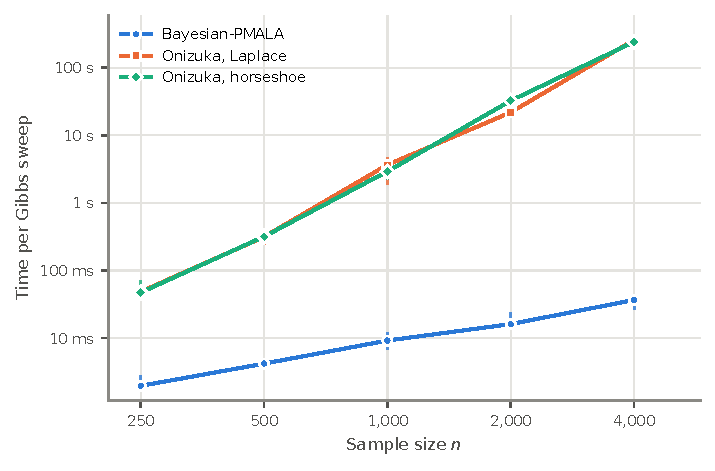
\includegraphics[width=0.7\textwidth]{figures/scal_time.pdf}
\caption{Median time per complete Gibbs sweep against sample size, log--log axes, with vertical bars spanning the range across replicates. The Onizuka samplers use \texttt{sparse = TRUE}. Values in Table~\ref{tab:cost_scaling}.}
\label{fig:cost_scaling}
\end{figure}

\paragraph{Results.} Table~\ref{tab:cost_scaling} and Figure~\ref{fig:cost_scaling} report the measurements. The time per sweep of Bayesian-PMALA is proportional to $n$: it costs between $7.8$ and $9.2$ microseconds per observation at every $n$, from $2.0$~ms per sweep at $n = 250$ to $36.6$~ms at $n = 4000$. A sweep of either Onizuka sampler takes about $48$~ms at $n = 250$, $0.3$~s at $n = 500$, $3$~s at $n = 1000$, $22$--$33$~s at $n = 2000$ and $4$ minutes at $n = 4000$. The two priors differ only in their scalar and local-scale updates and take the same time to within the replicate variation. The gap therefore widens with every doubling of $n$: an Onizuka sweep takes about $25$ times a Bayesian-PMALA sweep at $n = 250$, $75$ times at $n = 500$, $320$--$400$ times at $n = 1000$, $1\,400$--$2\,000$ times at $n = 2000$ and $6\,600$--$7\,000$ times at $n = 4000$.

\begin{figure}[!htbp]
\centering
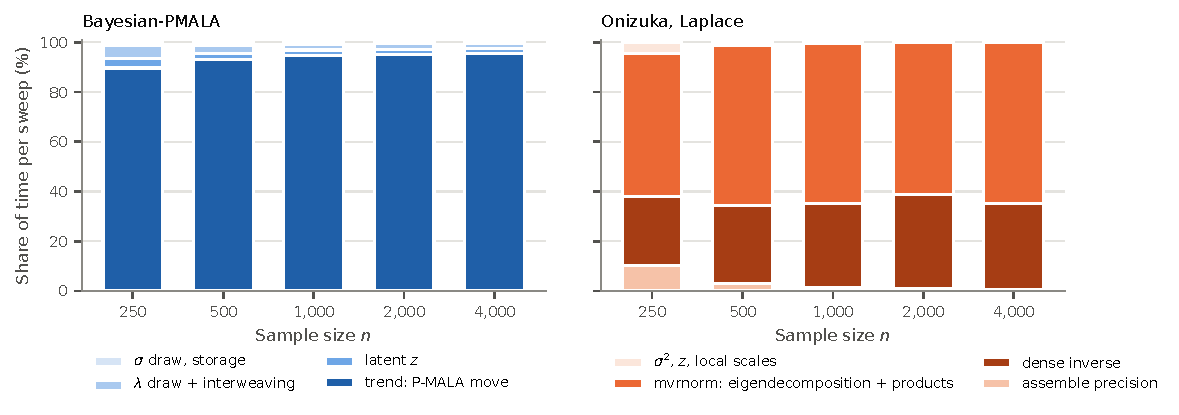
\includegraphics[width=\textwidth]{figures/scal_breakdown.pdf}
\caption{Share of the time per sweep spent in each update, median over replicates. Left: Bayesian-PMALA, where the P-MALA move comprises both proximal maps, the factorizations of the ADMM system and of the metric, the proposal noise and the acceptance ratio. Right: the Onizuka Laplace sampler with \texttt{sparse = TRUE}; the shares of the horseshoe sampler agree with these to within three percentage points at every $n$.}
\label{fig:cost_breakdown}
\end{figure}

\paragraph{Where the time goes.} Figure~\ref{fig:cost_breakdown} shows where the time of a sweep is spent. In Bayesian-PMALA the P-MALA move takes $90\%$ of the sweep at $n = 250$ and $96\%$ at $n = 4000$; the latent variables, the penalty with its interweaving step, and the scale take the rest, and the shares change little with $n$. In the Onizuka samplers the dense inverse takes $28$--$38\%$ of the sweep and \texttt{mvrnorm} $57$--$66\%$, together $85\%$ at $n = 250$ and $95$--$99\%$ for $n \ge 500$. Sparse assembly of the precision falls from $10\%$ of the sweep at $n = 250$ to under $1\%$ at $n = 4000$, and the updates of $\sigma^2$, the latent variables and the shrinkage parameters from $5\%$ to below $0.1\%$. Timed in isolation at $n = 2000$, the three dense steps of the trend draw take $12.0$~s for the inverse, $15.8$~s for the eigendecomposition and $4.4$~s for the product that forms the draw, consistent with the $22$--$42$~s per sweep in Table~\ref{tab:cost_scaling}.

\paragraph{Scope.} Because its time per observation is constant, the time per sweep of Bayesian-PMALA extends directly to longer series: at the $n = 8{,}640$ of the application in Section~\ref{sec:app:spod}, roughly $9$ microseconds per observation give about $80$~ms per sweep. Fitting several quantile levels multiplies the time of either method by the number of levels; the joint sampler of Section~\ref{subsec:joint} uses the same banded computations, with interior-point steps only when a neighbouring curve binds. The difference in running time belongs to the supplied implementation, not to the hierarchy of \citet{onizuka2024fast}. Its precision matrix is banded with half-bandwidth $k + 1$, so the Gaussian draw could be obtained from a banded Cholesky factorization; even a dense Cholesky draw from the same precision, without the explicit inverse and the eigendecomposition, took $1.1$~s at $n = 2000$ in the profile above, against $32$~s for the three steps of the supplied code. The comparison concerns time per sweep on one data set, one quantile level and one difference order; the efficiency of the chains per sweep is a separate question.
